\section{MIP bound: \therecord}

\label{mip_bound}


%\begin{figure}[H]
\begin{wrapfigure}[10]{R}{0.55\textwidth}
\centering
\vspace{-50pt}
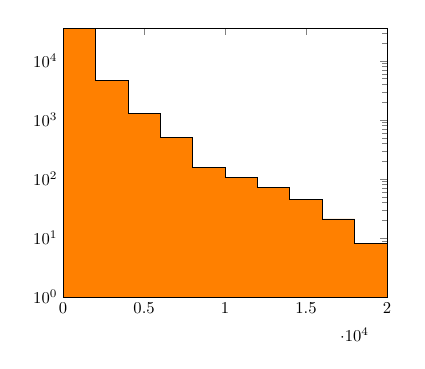
\begin{tikzpicture}[scale=0.6]
  \begin{semilogyaxis}[
    ymin=1,
    ymax=36033,
    log origin=infty,
    enlargelimits=false
  ]
    \addplot
      [const plot,fill=orange,draw=black]
      coordinates
        {(0,36033)    (2000,4644)  (4000,1302)   (6000,503)
         (8000,155) (10000,106)  (12000,71)  (14000,45)
         (16000,21) (18000,8)  (20000,1)}
  \closedcycle;
  \end{semilogyaxis}
\end{tikzpicture}
\caption{The vertical axis shows the number of cases and the horizontal axis shows the computation time in seconds. }
\label{histogram}
%\end{figure}
\end{wrapfigure}
Let us notice that results obtained in Theorem \ref{thm:linear_relax} can be naturally strengthened through longer computations. In practice, we were able to target 
%within two months of computations with three off--the--shelf Linux PC 
the objective 485. %\todo{Add more details about the machines and perhaps a graph with distribution of results (time). }


From Section \ref{linear_bound} we know all \theoctagons instances and their performance under relaxed (\ref{lp0})---(\ref{lp4}) linear problem. Apparently, out of all \theoctagons problems, \theinstances instances have the relaxed bound bigger or equal to 485. These are exactly the instances which must be treated by direct computations if we want to reduce the bound to 485. The total computation time for this target was approximately 310 days using the optimization software {\tt gurobi} (see \cite{gurobi}) on a single core of a Linux machine equipped with {\tt Intel\textsuperscript{\textregistered}} {\tt Xeon\textsuperscript{\textregistered}} {\tt CPU X3220@2.40GHz} with 8GB of RAM. The graph \ref{histogram} shows on the logarithmic scale the distribution of the computation time among \theinstances instances\footnote{In fact, a half of the instances required less than 100~sec. to reach the limit of \therecord and 9 instances required the computation time longer than 18000 seconds.}. 
